\section{Лекция №12 (18.12.2023)}

\subsection{UDP (User Datagram Protocol)}

Протокол транспортного уровня без установления соединения. Используется для пересылки стримов.

\begin{figure}[!htb]
    \centering
    \vphantom{\small1}
    \begin{bytefield}[bitwidth=0.03125\linewidth,bitformatting={\small}]{32}
        \bitheader{0,16,31}\\
        \bitbox{16}{Порт источника} & \bitbox{16}{Порт назначения}\\
        \bitbox{16}{Длина сегмента} & \bitbox{16}{Контрольная сумма}
    \end{bytefield}
    \caption{Заголовок сегмента UDP}
    \label{img:udp}
\end{figure}

\subsection{DNS (Domain Name System)}

Протокол прикладного уровня. Основное (но не единственное!) предназначение протокола~--- преобразовать доменное имя в IP-адрес. Работает по UDP (53 порт).

Раньше все доменные имена были одноуровневыми. Для того, чтобы связать их с IP-адресами, использовался файл \texttt{hosts}. Сейчас DNS~--- распределенная база данных, построенная по принципу иерархии.

\image
{.75\textwidth}
{12/notes/inc/dns-hierarchy}
{DNS}

В DNS сервер знает только о нижележащем уровне: например, корневой сервер знает только о ru-, com- и edu-серверах.

DNS-сервера могут иметь кэш, который хранит записи вне зоны ответственности
сервера: например, сервер bmstu может хранить адрес iu7.vk.com. Срок хранения
записи в кэше определяется владельцем этой записи.

Поиск записи может быть осуществлен при помощи двух алгоритмов: рекурсивного и нерекурсивного.

\begin{figure}[H]
    \centering
    \begin{subfigure}{0.45\textwidth}
        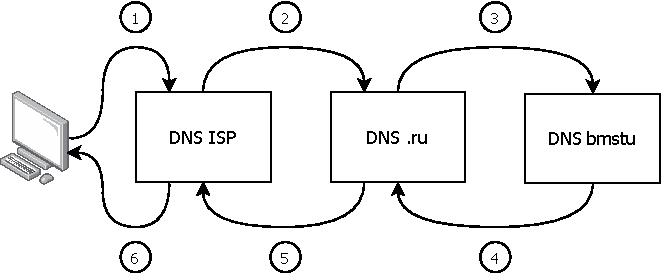
\includegraphics[width=\textwidth]{12/notes/inc/dns-recursive}
        \caption{Рекурсивный алгоритм}
    \end{subfigure}
    \hspace{.5cm}
    \begin{subfigure}{0.45\textwidth}
        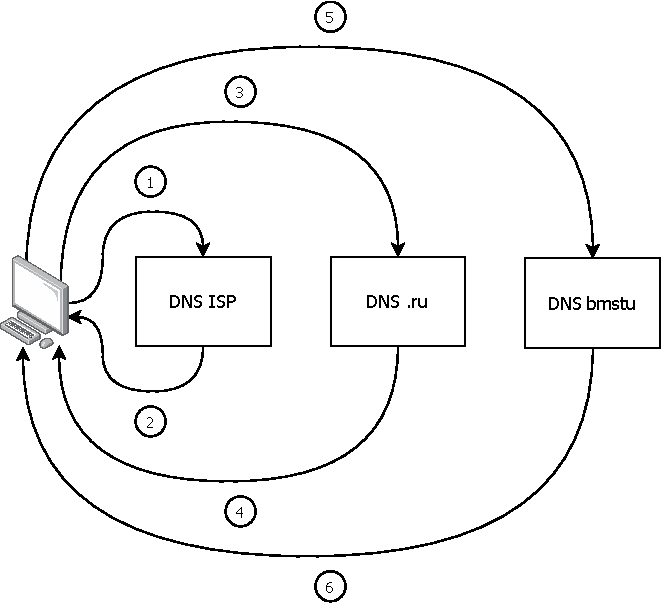
\includegraphics[width=\textwidth]{12/notes/inc/dns-non-recursive}
        \caption{Нерекурсивный алгоритм}
    \end{subfigure}
\end{figure}

\begin{figure}[!htb]
    \centering
    \vphantom{\small1}
    \begin{bytefield}[bitwidth=0.03125\linewidth,bitformatting={\small}]{32}
        \bitheader{0,16,31}\\
        \wordbox[lrt]{1}{Name}\\
        \skippedwords\\
        \wordbox[lrb]{1}{}\\
        \bitbox{16}{Type} & \bitbox{16}{Class}\\
        \bitbox{32}{TTL}\\
        \bitbox{16}{Resource Data Length} & \bitbox[lrt]{16}{}\\
        \wordbox[lrb]{1}{Resource Data}
    \end{bytefield}
    \caption{Запись DNS}
    \label{img:dns}
\end{figure}

Поля записи DNS:

\begin{enumerate}
    \item \textbf{Имя}. По сути~--- доменное имя.
    \item \textbf{Тип}. Функционал записи. Наиболее распространенные:
          \begin{itemize}
              \item record A~--- преобразует доменное имя в IPv4;
              \item record AAAA~--- преобразует доменное имя в IPv6;
              \item record CNAME~--- каноническое имя;
              \item record NS~--- сервер, ответственный за разрешение запросов для определенного
                    имени хоста.
          \end{itemize}
    \item \textbf{Класс}. На случай, если будет использоваться отличный от TCP/IP стек.
    \item \textbf{Time to Live}. Время, в течение которого разрешено хранить запись в кэше неответственного сервера.
    \item \textbf{Длина поля данных}. Измеряется в байтах.
    \item \textbf{Поле данных}. В зависимости от типа содержимое может отличаться.
\end{enumerate}

\subsection{SMTP (Simple Mail Transfer Protocol)}

По этому протоколу почту можно отправить, но не получить. Работает по TCP (25 порт).

Последовательность действий при работе SMTP:

\begin{enumerate}
    \item Установление TCP-соединения.
    \item <<Приветствие>> сервера~--- \texttt{HELO}.
    \item Авторизация~--- логин, пароль в base64.
    \item \texttt{MAIL FROM: <xxx@bmstu.ru>}.
    \item \texttt{RCPT TO: <yyy@bmstu.ru>}.
    \item \texttt{DATA}\\
          bla bla bla$\dlsh$\\
          .$\dlsh$
    \item \texttt{QUIT}.
\end{enumerate}

Сервер отвечает кодом из трех цифр и текстом. Первая цифра определяет функционал:

\begin{itemize}
    \item 2~--- <<все хорошо>>;
    \item 3~--- идет процесс: например, при помощи этого кода сервер сообщит о готовности считать пароль после ввода логина;
    \item 5~--- <<все плохо>>: например, ошибка авторизации.
\end{itemize}

Вторые две цифры добавляют конкретику.

\begin{center}
    \texttt{\underline{2}\,\underline{5}\,\underline{0} \underline{OK}}\\
    \texttt{\underline{3}\,\underline{\phantom{5}}\,\underline{\phantom{5}} \underline{\phantom{OK}}}\\
    \texttt{\underline{5}\,\underline{\phantom{5}}\,\underline{\phantom{5}} \underline{\phantom{OK}}}
\end{center}

\subsection{POP3 (Post Office Protocol)}

Первый из двух протоколов получения почты. Работает по TCP (110 порт).

В отличие от SMTP сервер может ответить одним из двух сообщений:

\begin{itemize}
    \item \texttt{+OK};
    \item \texttt{-ERR \underline{\phantom{reason}}}.
\end{itemize}

Существует три режима работы с сервером POP3:

\begin{enumerate}
    \item \textbf{Авторизация}. Ввод логина и пароля в открытом (!) виде.
    \item \textbf{Передача}. Работа с письмами: подсчет количества писем, их размера (в символах!), чтение (по порядковому номеру). Можно также поставить <<галочку>> у писем, которые необходимо удалить. Само удаление произойдет в режиме обновления.
    \item \textbf{Обновление}. Запускается после команды \texttt{QUIT}.
\end{enumerate}

\subsection{IMAP (Internet Message Access Protocol)}

Второй протокол получения почты. Работает по TCP (143 порт).

POP3 предоставляет возможность работы с почтой на клиенте, а IMAP~--- на
сервере: в первом случае изменения между клиентами не синхронизируются.

POP3 хорош при плохом интернет-соединении.

\subsection{FTP (File Transfer Protocol)}

Протокол передачи файлов. Для корректной работы необходимо два TCP-соединения: для передачи команд и данных. Последнее <<живет>> ровно одну транзакцию.

\image
{\textwidth}
{12/notes/inc/ftp}
{Схема работы FTP}

Здесь:

\begin{itemize}
    \item PI~--- Protocol Interpreter;
    \item DTP~--- Data Transfer Process.
\end{itemize}

Номер порта для соединения для передачи данных на сервере зависит от режима работы: активный~--- 20 порт, пассивный~--- <<высокий>> порт.

\begin{figure}[H]
    \centering
    \begin{subfigure}{0.45\textwidth}
        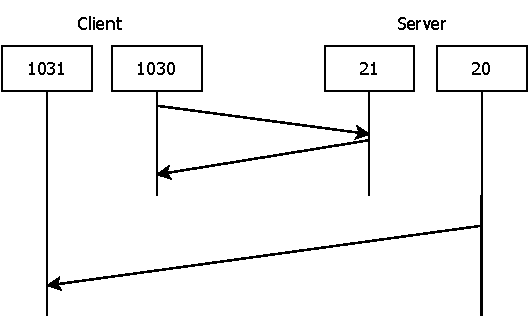
\includegraphics[width=\textwidth]{12/notes/inc/ftp-active}
        \caption{Активный режим (соединение для передачи данных открывает сервер)}
    \end{subfigure}
    \hspace{.5cm}
    \begin{subfigure}{0.45\textwidth}
        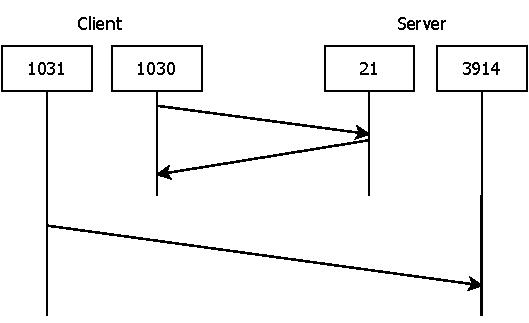
\includegraphics[width=\textwidth]{12/notes/inc/ftp-passive}
        \caption{Пассивный режим (соединение для передачи данных открывает клиент)}
    \end{subfigure}
\end{figure}

Может возникнуть проблема с брандмауэром: попытка открыть соединение с 20 порта сервера на высокий порт клиента будет заблокирована.

Есть три разновидности команд в FTP:

\begin{enumerate}
    \item \textbf{Управление доступом}. Логин, пароль (в открытом виде), ограничение прав доступа к папкам.
    \item \textbf{Управление потоком}. Команды, которые управляют параметрами TCP-соединения для передачи данных. Можно указать режим работы сервера, номера портов.
    \item \textbf{FTP-сервис}. Команды, предназначенные для работы с файлами.
\end{enumerate}

\subsection{Telnet}

Используется для удаленного управления устройством. Работает по TCP (23 порт).

Telnet может работать в нескольких режимах:

\begin{enumerate}
    \item \textbf{Полудуплексный}. Отображение печатаемых символов происходит на клиенте, а их отправка на удаленное устройство~--- по команде от удаленного устройства \texttt{GO AHEAD}.
    \item \textbf{Символьный}. Печатаемый символ отправляется на удаленное устройство, применяется там, возвращается на клиент и только после этого отображается.
    \item \textbf{Условно строчный}. Появился в результате ошибки программиста. Нет эхо-печати: печатаемые символы не отображаются. Строка отправляется по нажатию Enter.
    \item \textbf{Строчный}. Печатаемый символ сразу отображается на клиенте, а отправка команды осуществляется по нажатию Enter.
\end{enumerate}

Telnet не следует использовать за пределами локальной сети из соображений
безопасности~--- лучше использовать SSH.

\subsection{HTTP}

Работает по TCP (80 порт).

HTTP поддерживает два вида соединений:

\begin{enumerate}
    \item \textbf{Непостоянное}. Для скачивания каждого объекта запрашиваемой страницы открывается отдельное TCP-соединение.
    \item \textbf{Постоянное}. Страница и ее объекты скачиваются в рамках одного TCP-соединения. Может быть двух видов:
          \begin{enumerate}
              \item \textbf{Без конвейеризации}. Сервер простаивает в ожидании запроса на следующий объект.
              \item \textbf{С конвейеризацией}. Все запросы на все объекты формируются сразу: как только сервер ответил на первый запрос, в его буфере уже содержится следующий запрос, который он начинает обрабатывать.
          \end{enumerate}
\end{enumerate}

В заголовке Content-Type содержится информация, необходимая для корректного отображения ответа. Используется стандарт MIME (Multipurpose Internet Mail Extensions).